\section{Methodology}

\subsection{Environment Implementation}

We implemented a custom Flappy Bird environment that faithfully reproduces the mechanics of the original game while providing the necessary interfaces for reinforcement learning. The environment is structured as a physics-based simulation where a bird avatar must navigate through gaps between pairs of pipes that scroll horizontally across the screen. The simulation runs at 30 frames per second, consistent with most game implementations, to provide a smooth visual experience while allowing sufficient time for the agent to process and respond to the environment state.

The bird's movement follows simplified physics: it experiences constant downward acceleration due to gravity, and flapping provides an instantaneous upward velocity. The pipes are generated with random heights but maintain a constant gap size between the upper and lower segments. The horizontal distance between consecutive pipe pairs remains fixed, creating a regular pattern of obstacles that increases the game's predictability while still requiring precise control.
\begin{figure}[!t]
\centering
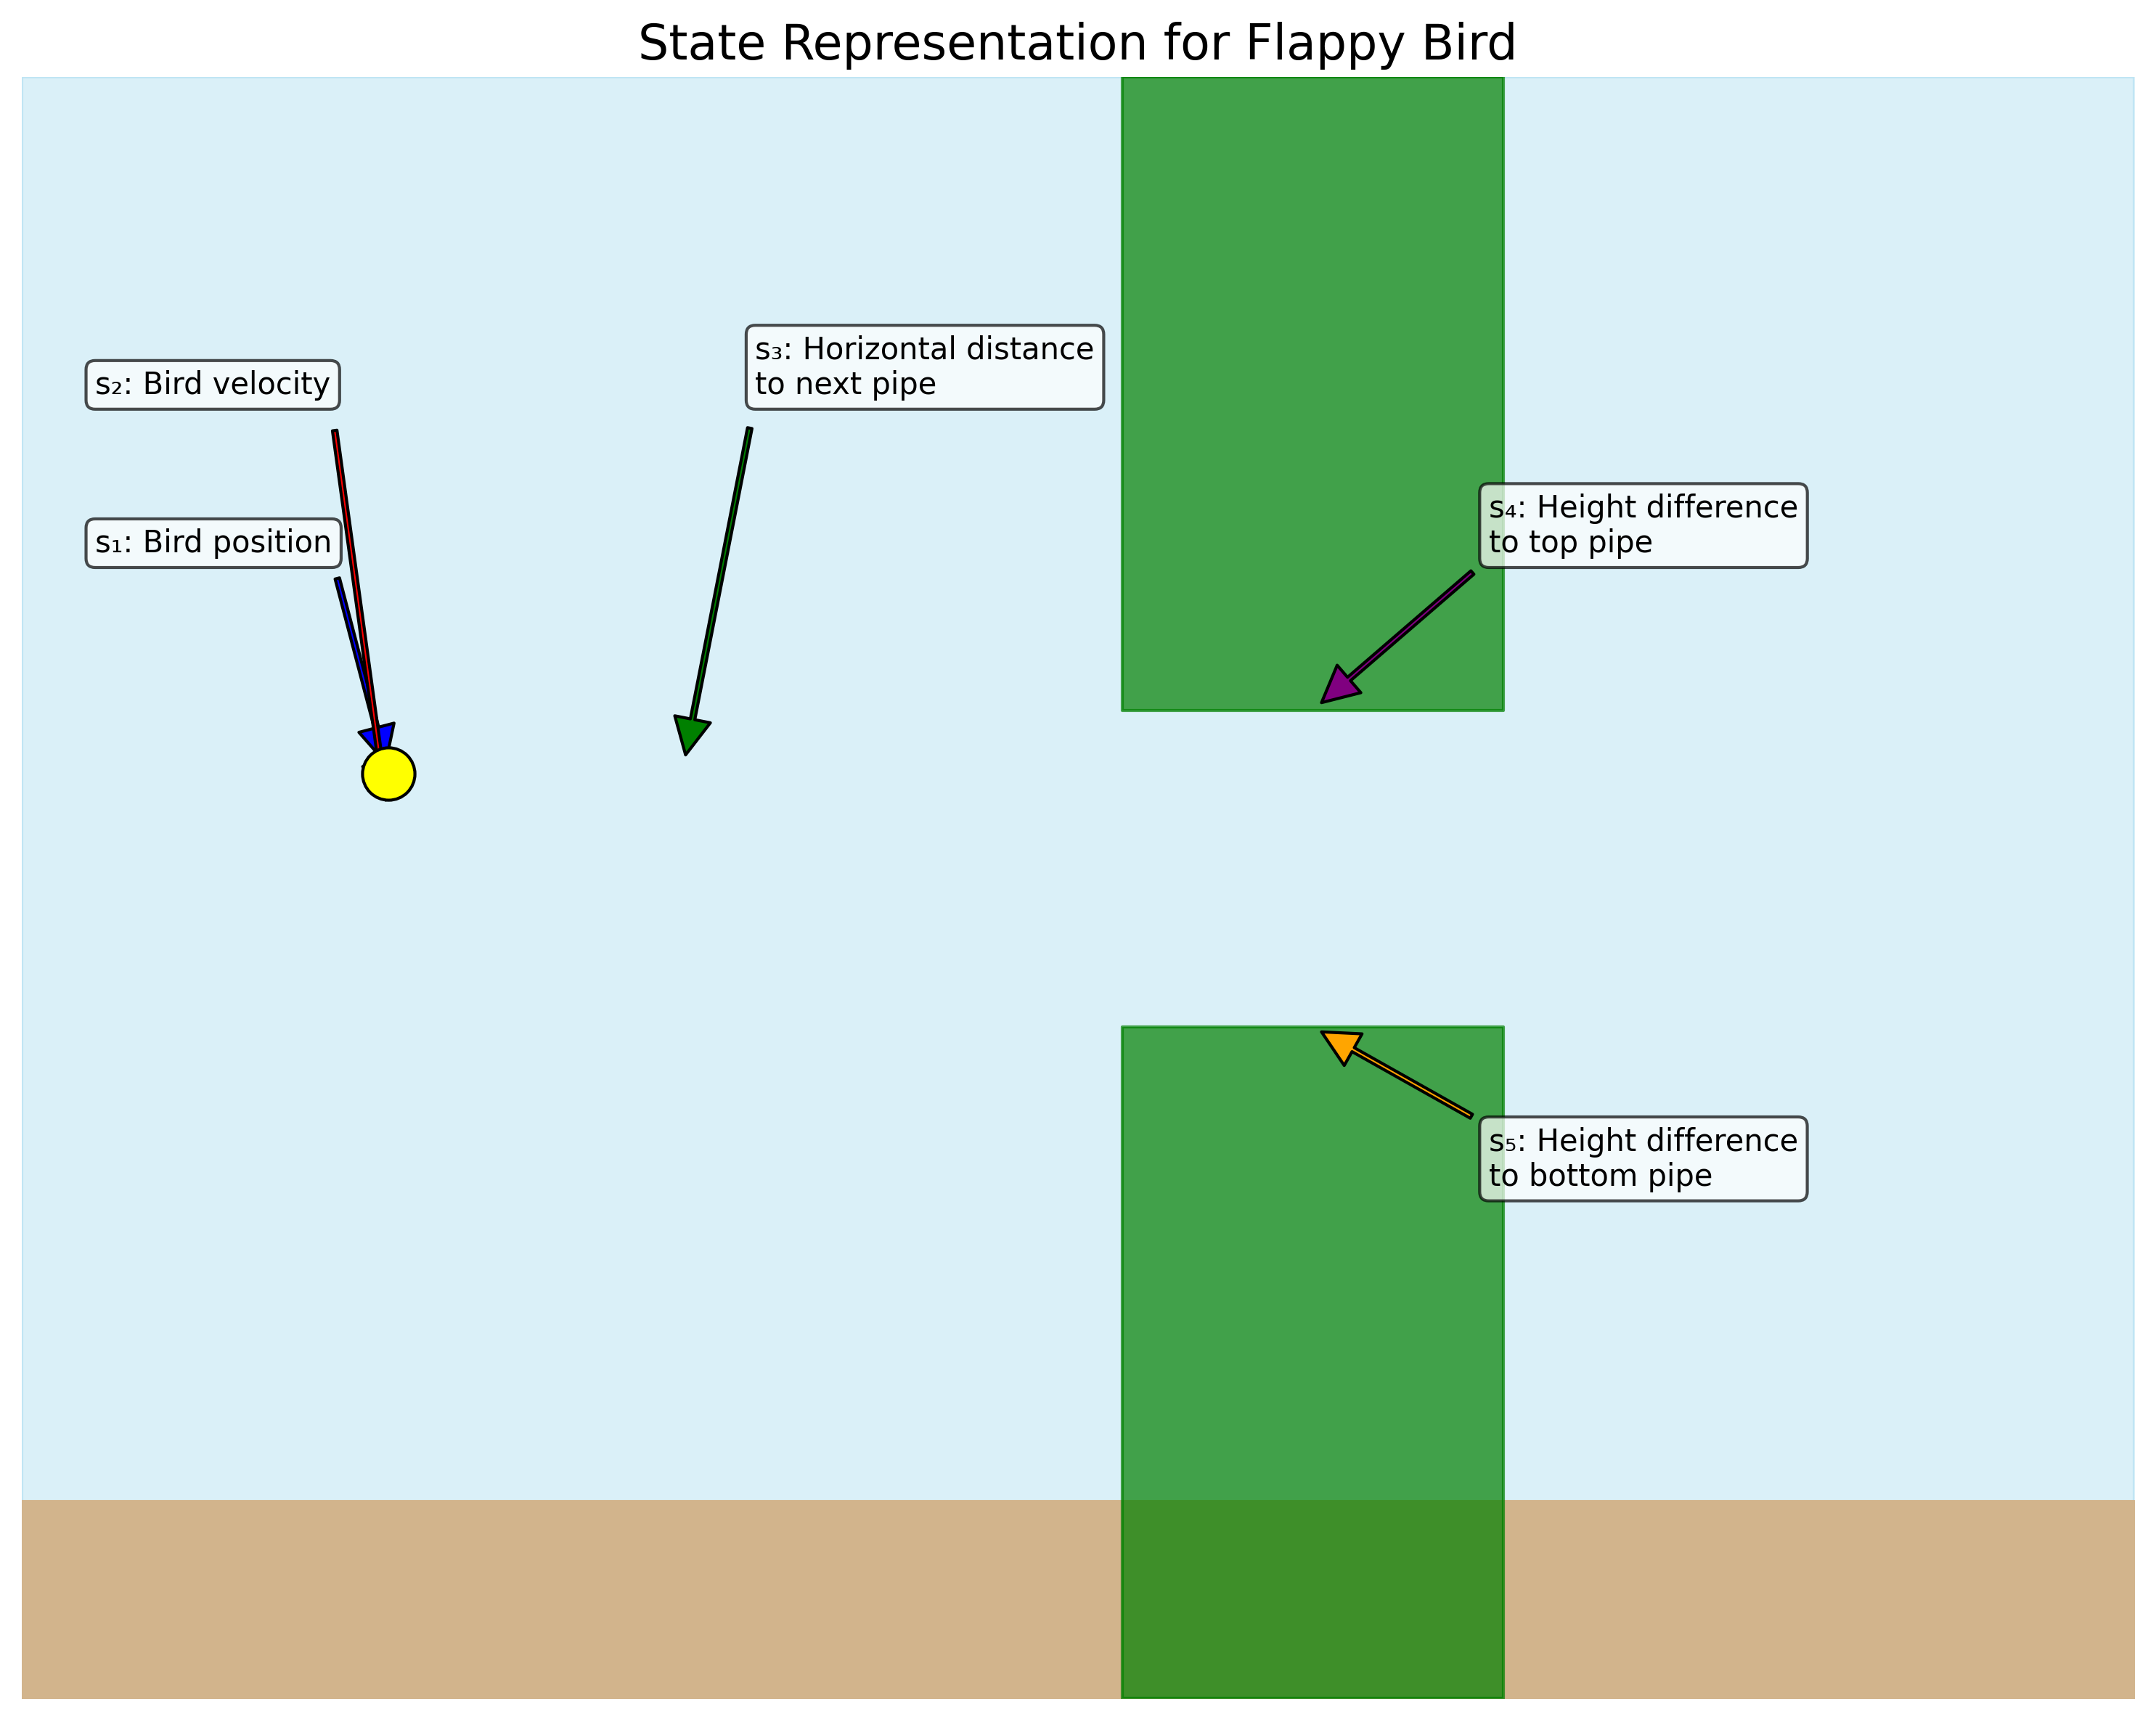
\includegraphics[width=\columnwidth]{/Users/admin/GitHUb/Flappy_Bird_RL/Flappy_Bird_RL/Figures/state_representation.png}
\caption{State representation used by the DQN agent, consisting of five normalized features: (s₁) bird's vertical position, (s₂) bird's vertical velocity, (s₃) horizontal distance to the next pipe, (s₄) height difference to top pipe, and (s₅) height difference to bottom pipe.}
\label{fig:state_representation}
\end{figure}
Unlike previous implementations that rely on pixel-based representations \cite{yang2023foundation}, we employed a compact state representation consisting of five normalized features: (1) the bird's vertical position, (2) the bird's vertical velocity, (3) the horizontal distance to the next pipe, (4) the height difference between the bird and the top pipe, and (5) the height difference between the bird and the bottom pipe. This representation provides sufficient information for decision-making while significantly reducing the input dimensionality, allowing for more efficient learning compared to pixel-based approaches.
\begin{figure}[!t]
\centering
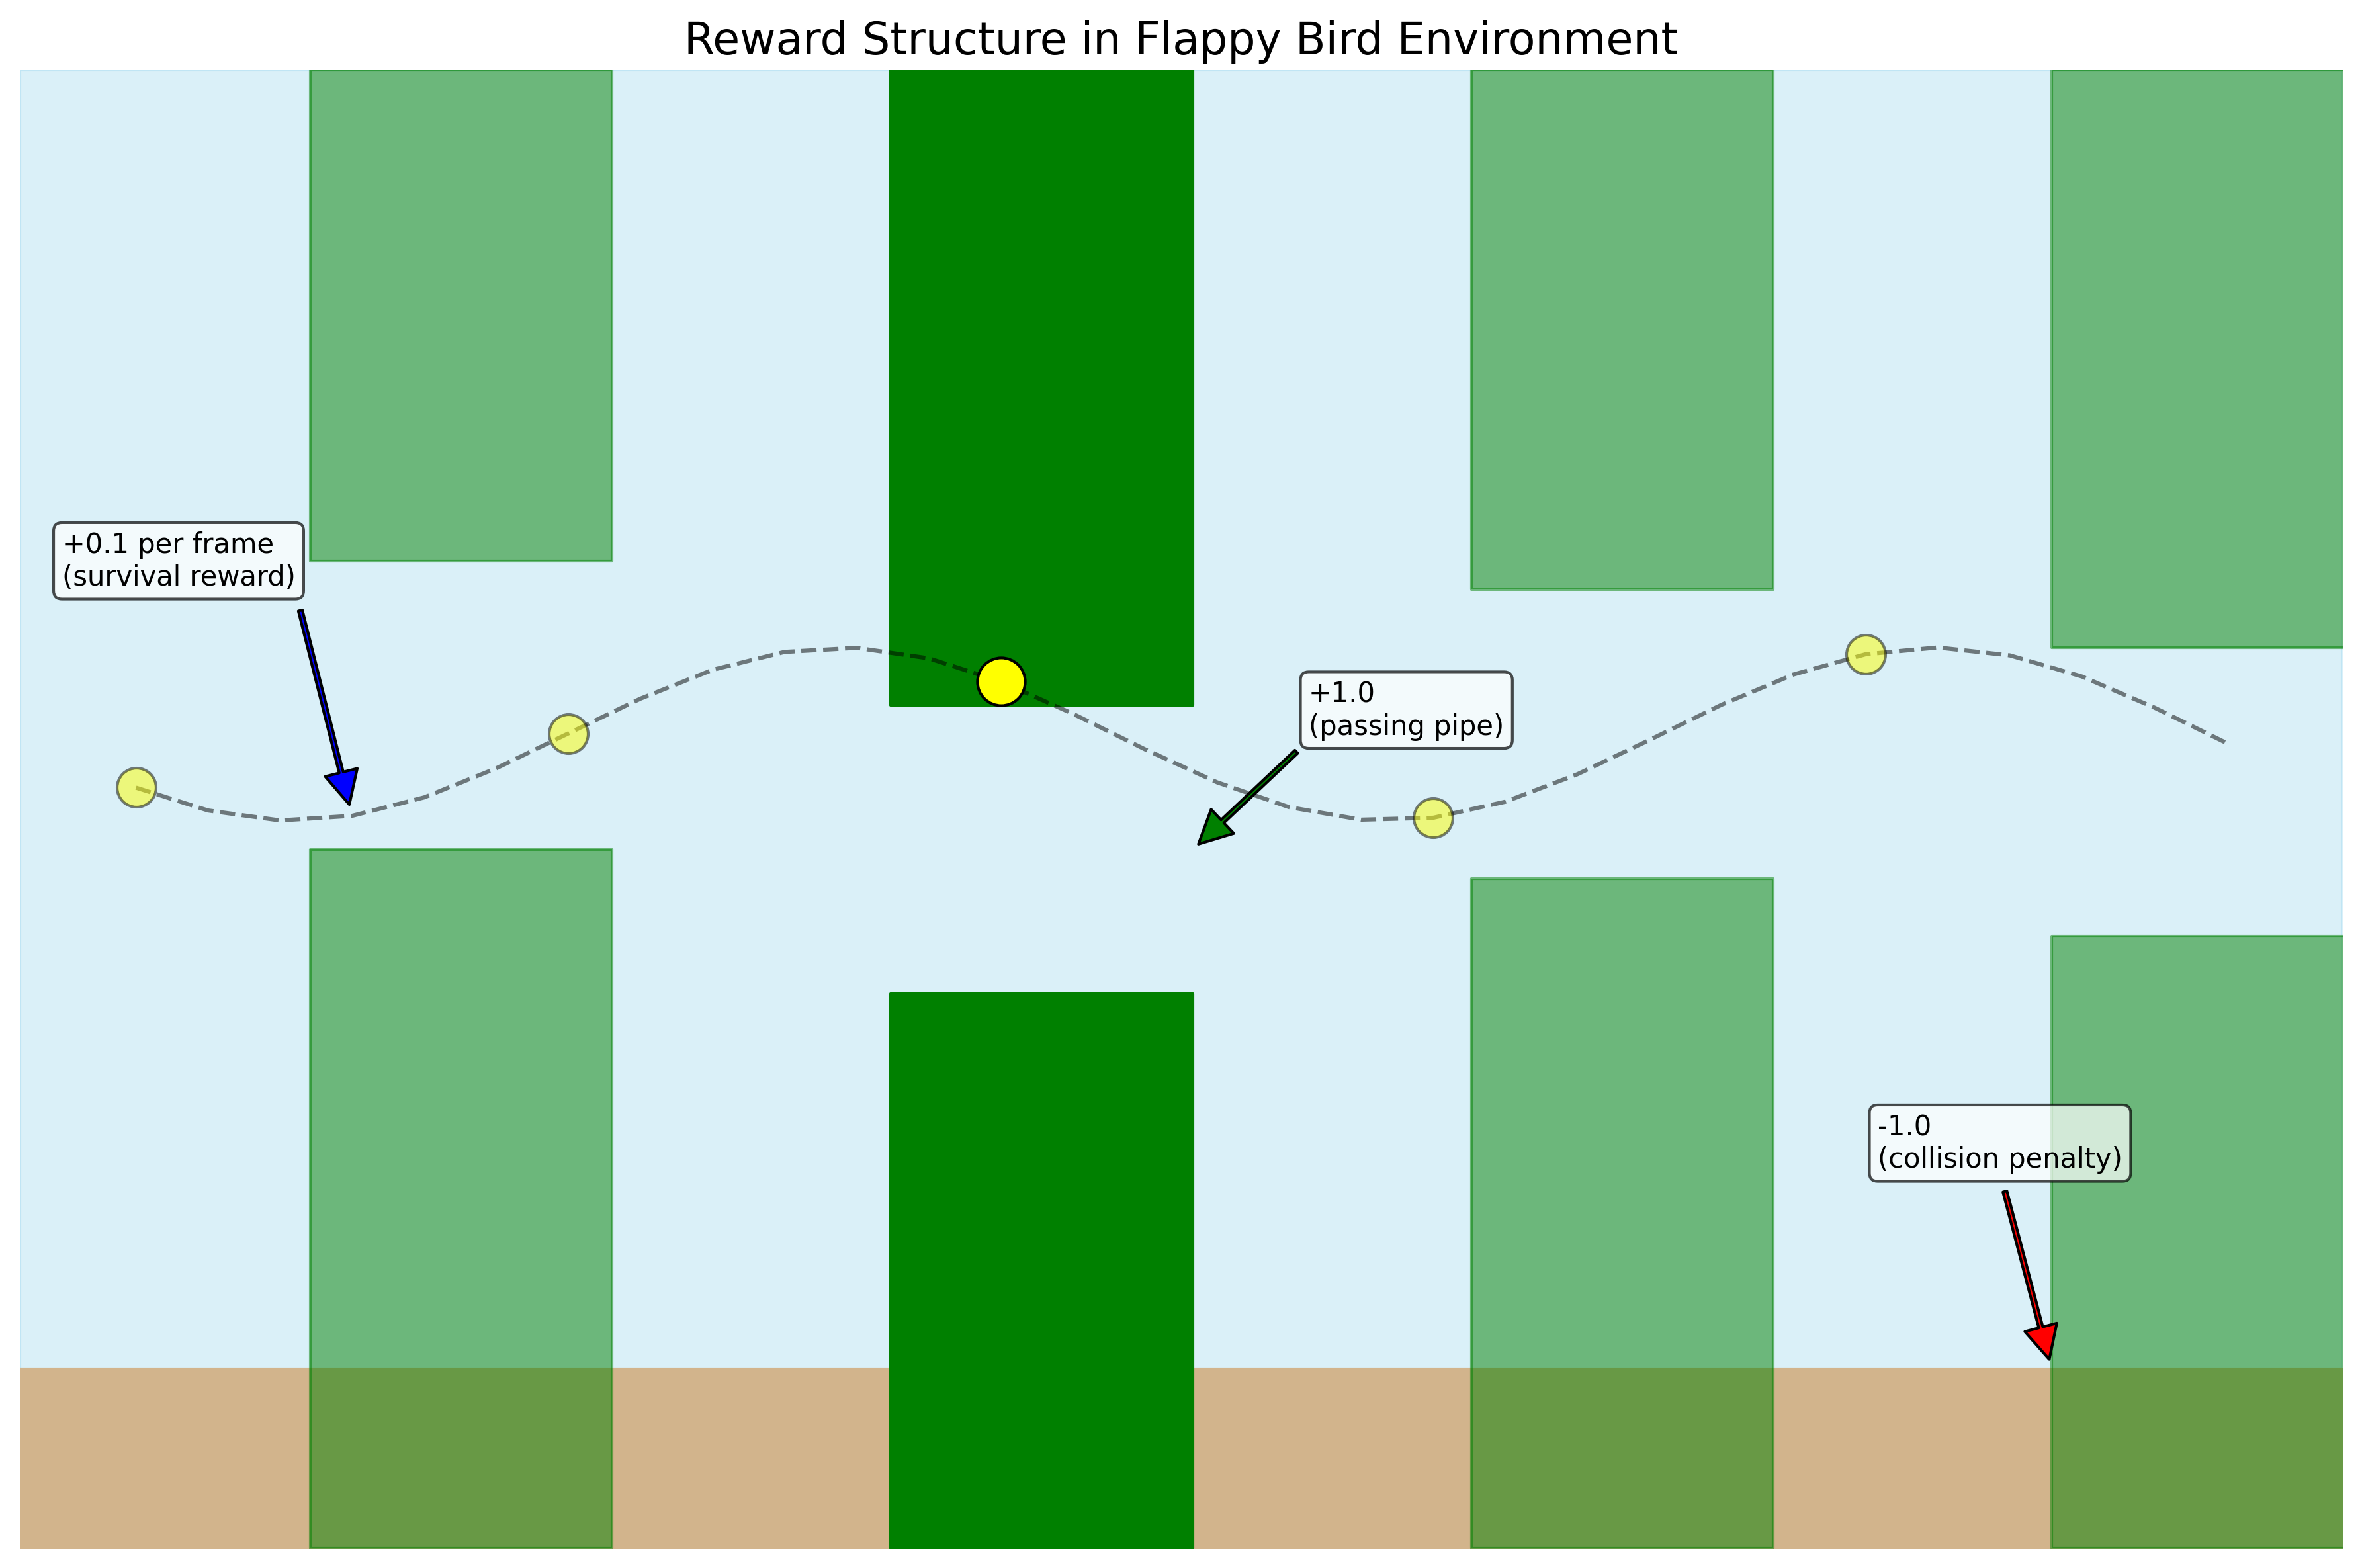
\includegraphics[width=\columnwidth]{/Users/admin/GitHUb/Flappy_Bird_RL/Flappy_Bird_RL/Figures/reward_structure.png}
\caption{Reward structure in the Flappy Bird environment: small positive reward (+0.1) for each frame survived, larger reward (+1.0) for successfully passing through a pipe, and negative reward (-1.0) for collisions.}
\label{fig:reward_structure}
\end{figure}
The action space consists of two discrete actions: "do nothing" (allowing the bird to fall under gravity) and "flap" (giving the bird an upward velocity impulse). This binary action space aligns with the original game mechanics and creates a clear decision boundary for the agent to learn.
\begin{figure}[!t]
\centering
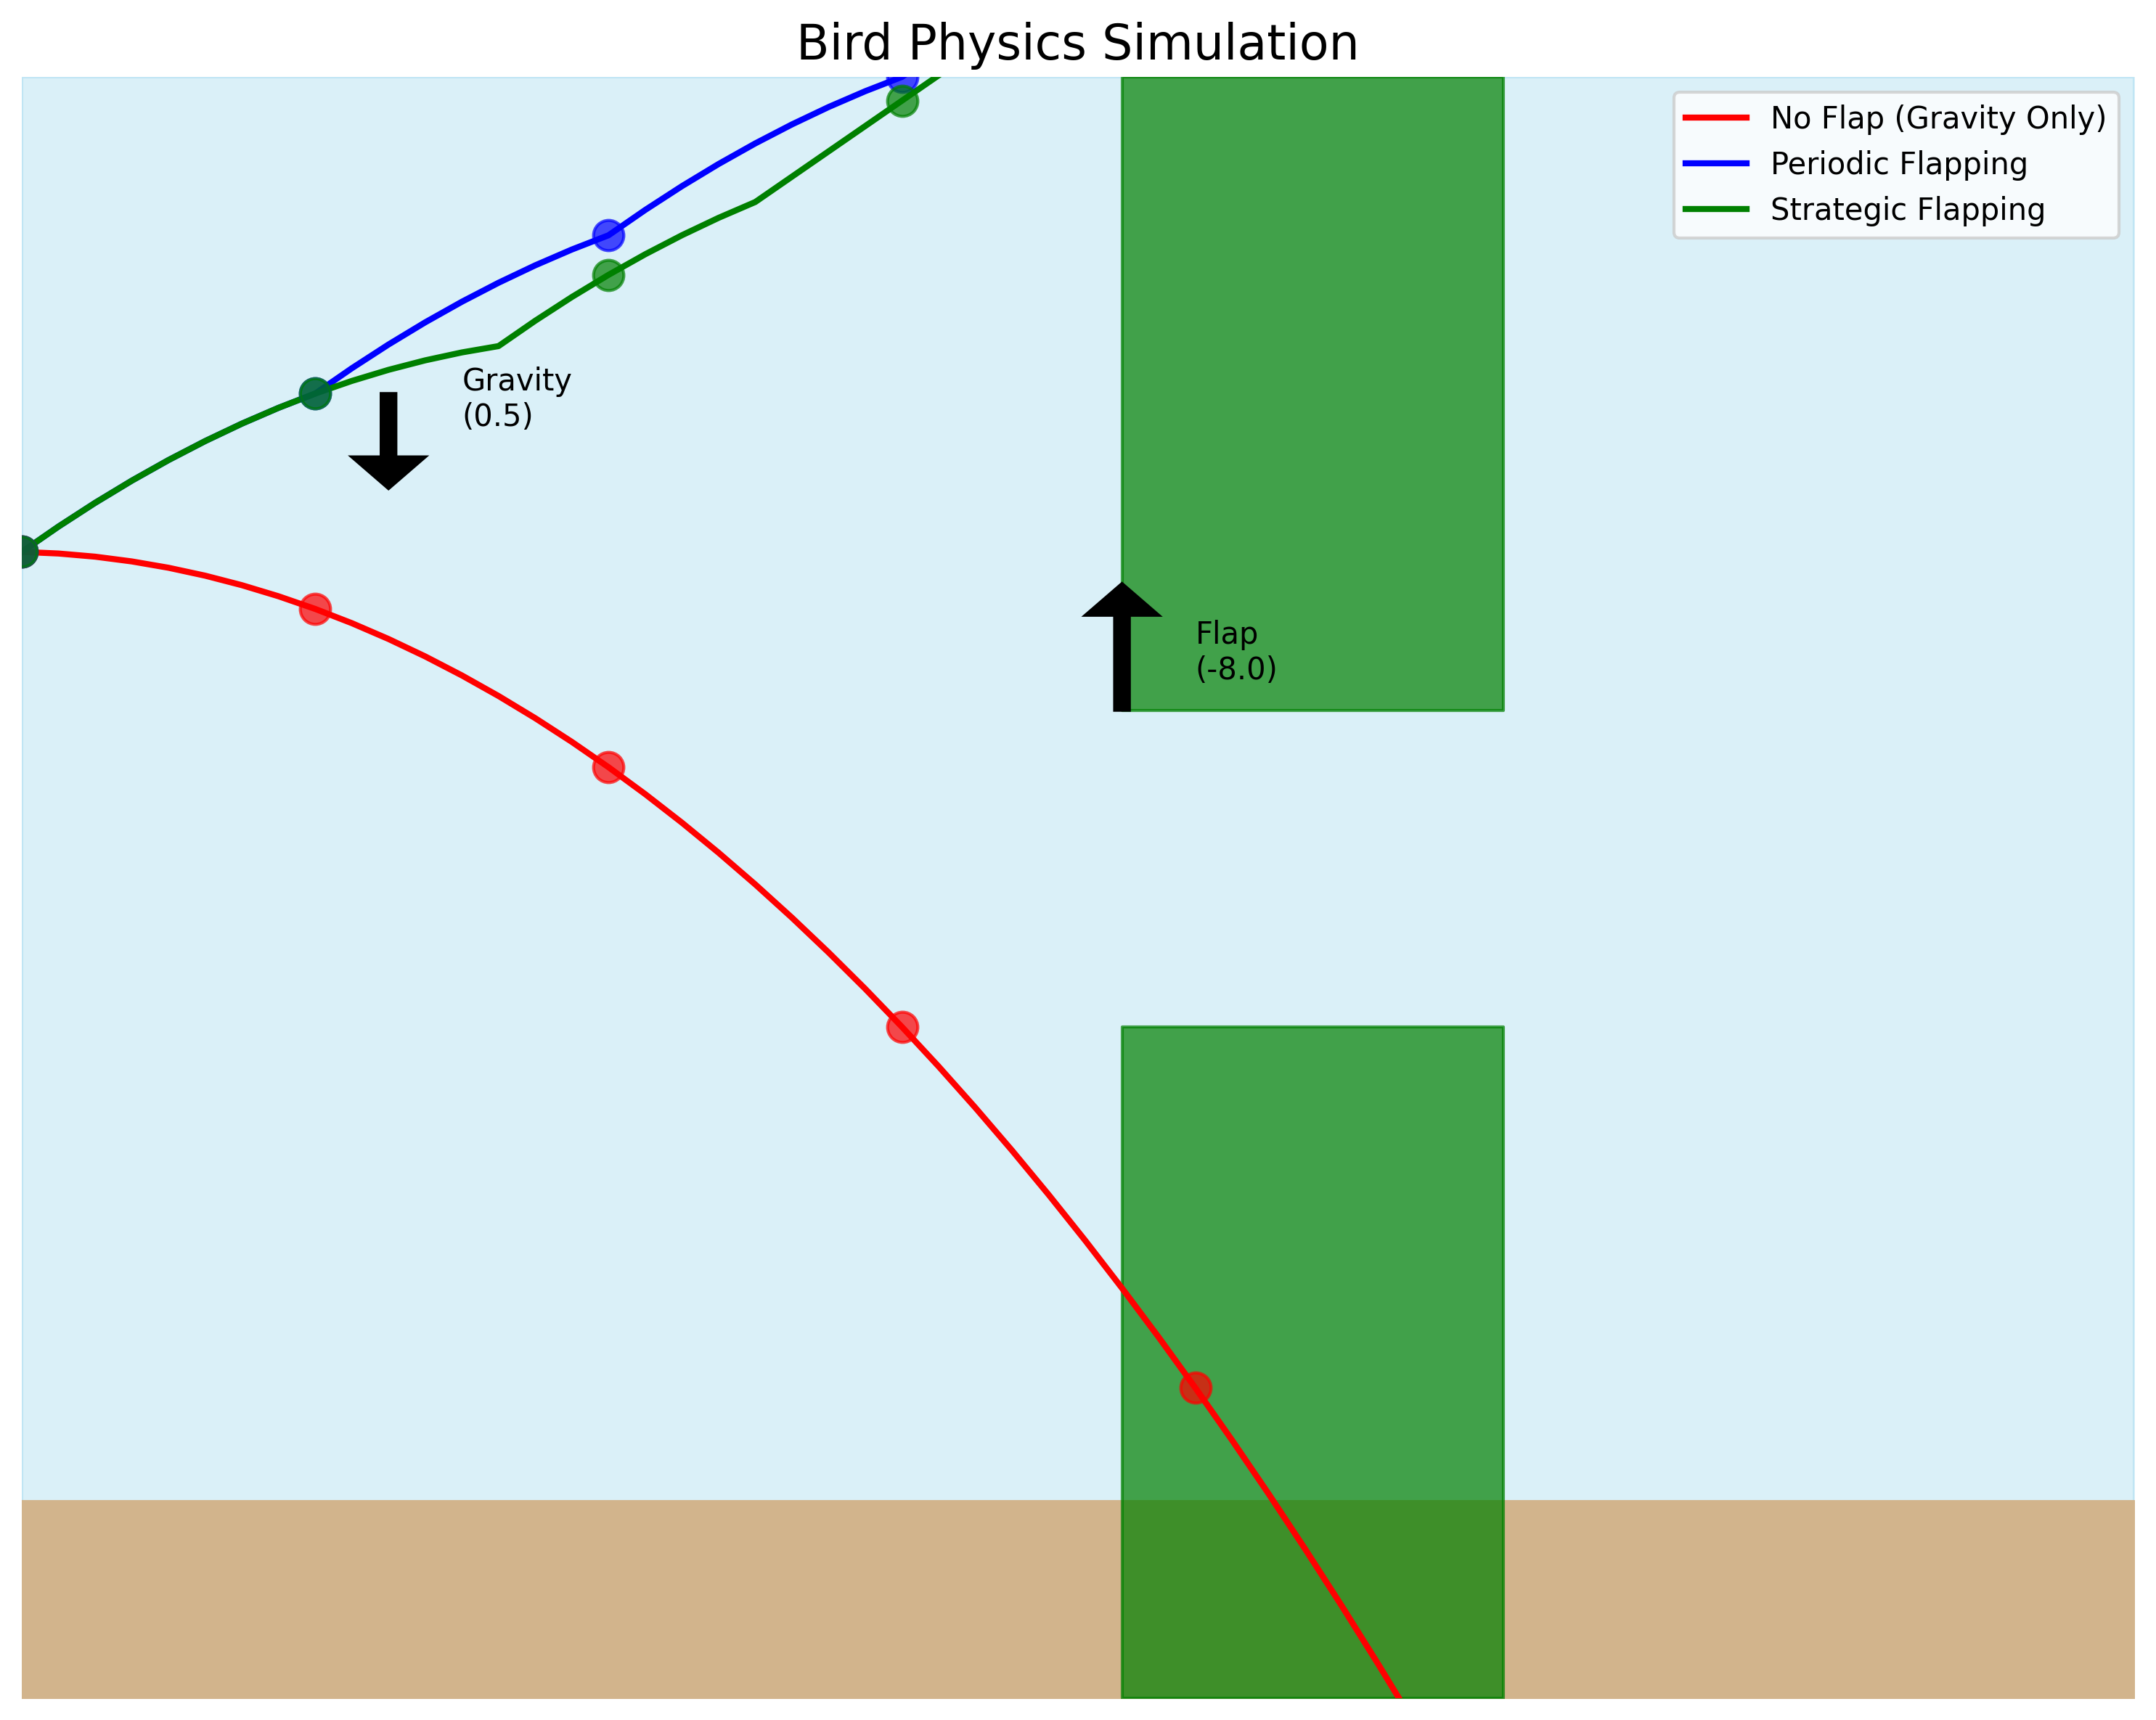
\includegraphics[width=\columnwidth]{/Users/admin/GitHUb/Flappy_Bird_RL/Flappy_Bird_RL/Figures/bird_physics.png}
\caption{Bird flight trajectory simulation showing three strategies: no flapping (gravity only, red line), periodic flapping (blue line), and strategic flapping (green line). The gravity constant (0.5) pulls the bird downward while each flap provides an upward velocity (-8.0).}
\label{fig:bird_physics}
\end{figure}
We designed the reward function to provide meaningful feedback that guides the learning process toward successful gameplay. The agent receives a small positive reward (+0.1) for each frame it survives, encouraging longevity, a larger reward (+1.0) for successfully navigating through a pipe, and a negative reward (-1.0) for collisions. This reward structure balances immediate feedback with the long-term objective of maximizing the game score.
\begin{figure}[!t]
\centering
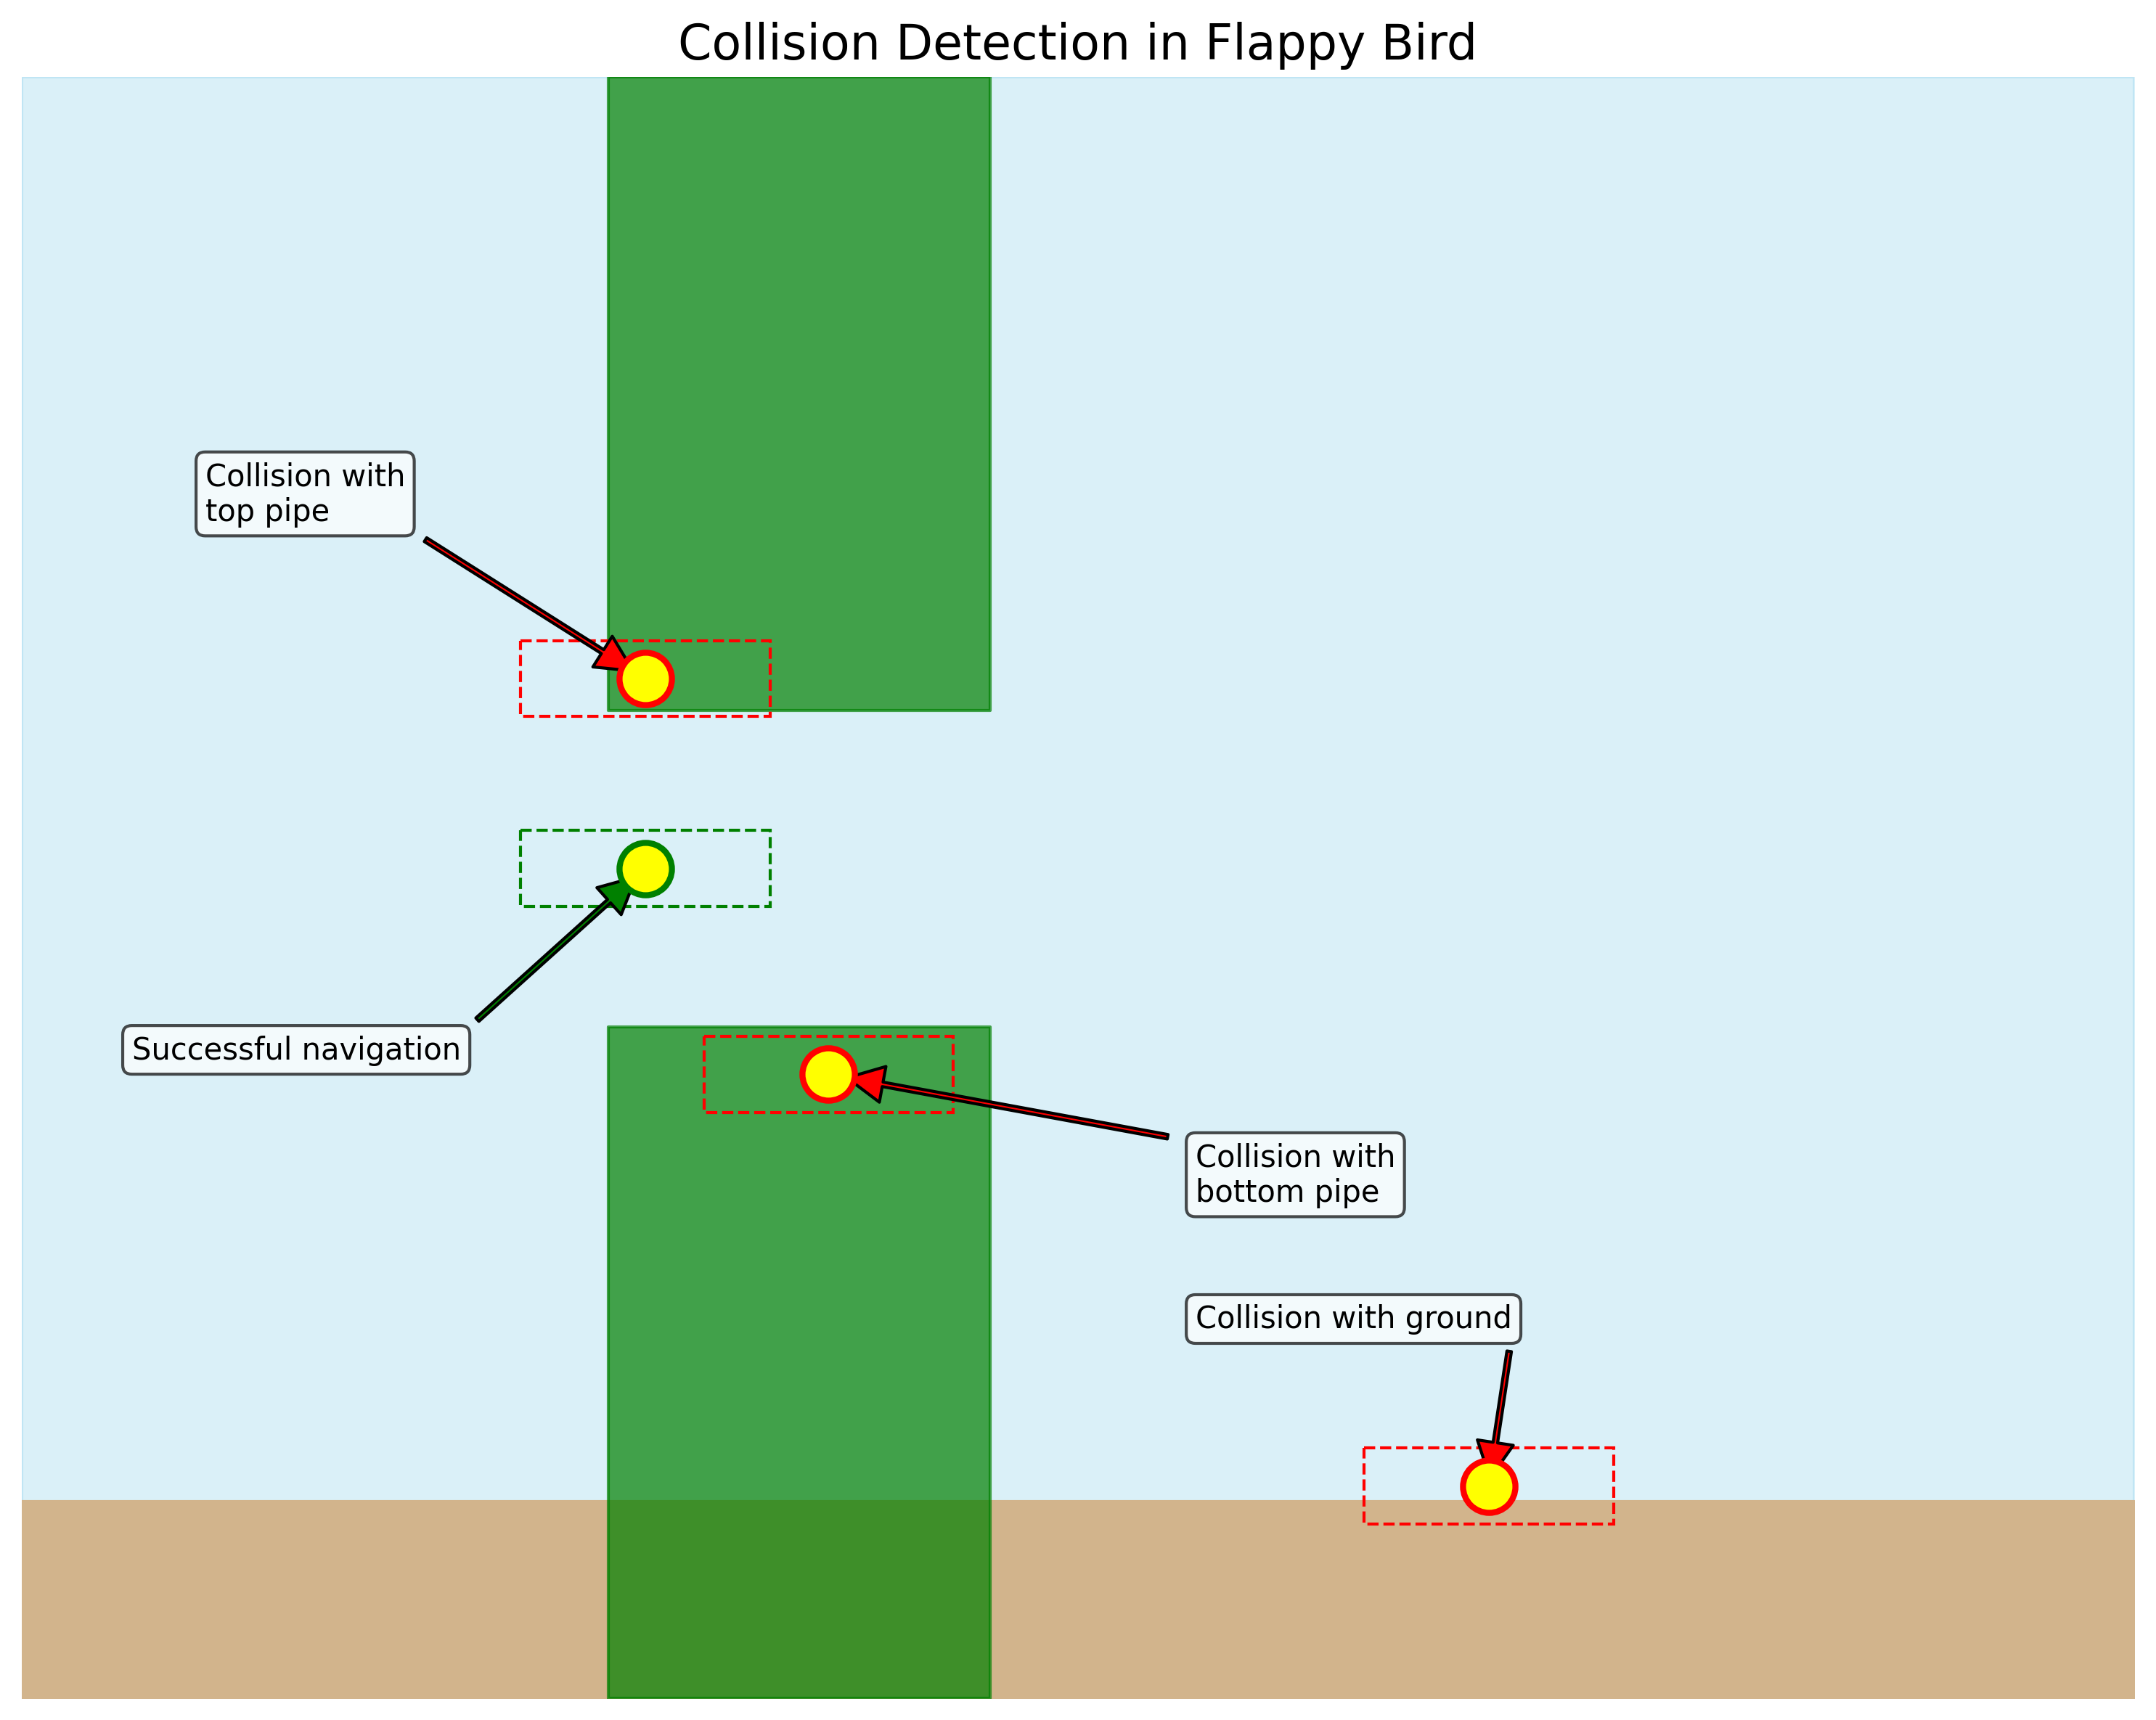
\includegraphics[width=\columnwidth]{/Users/admin/GitHUb/Flappy_Bird_RL/Flappy_Bird_RL/Figures/collision_detection.png}
\caption{Collision detection mechanism showing different scenarios: collision with top pipe, collision with bottom pipe, collision with ground, and successful navigation through pipe gap.}
\label{fig:collision_detection}
\end{figure}
\subsection{Neural Network Architecture}

Our DQN implementation employs a feedforward neural network architecture implemented in PyTorch. The network consists of an input layer corresponding to the five state features, followed by three hidden layers with 64, 64, and 32 neurons respectively, each using Rectified Linear Unit (ReLU) activation functions. The output layer contains two neurons corresponding to the Q-values for each possible action.
\begin{figure}[!t]
\centering
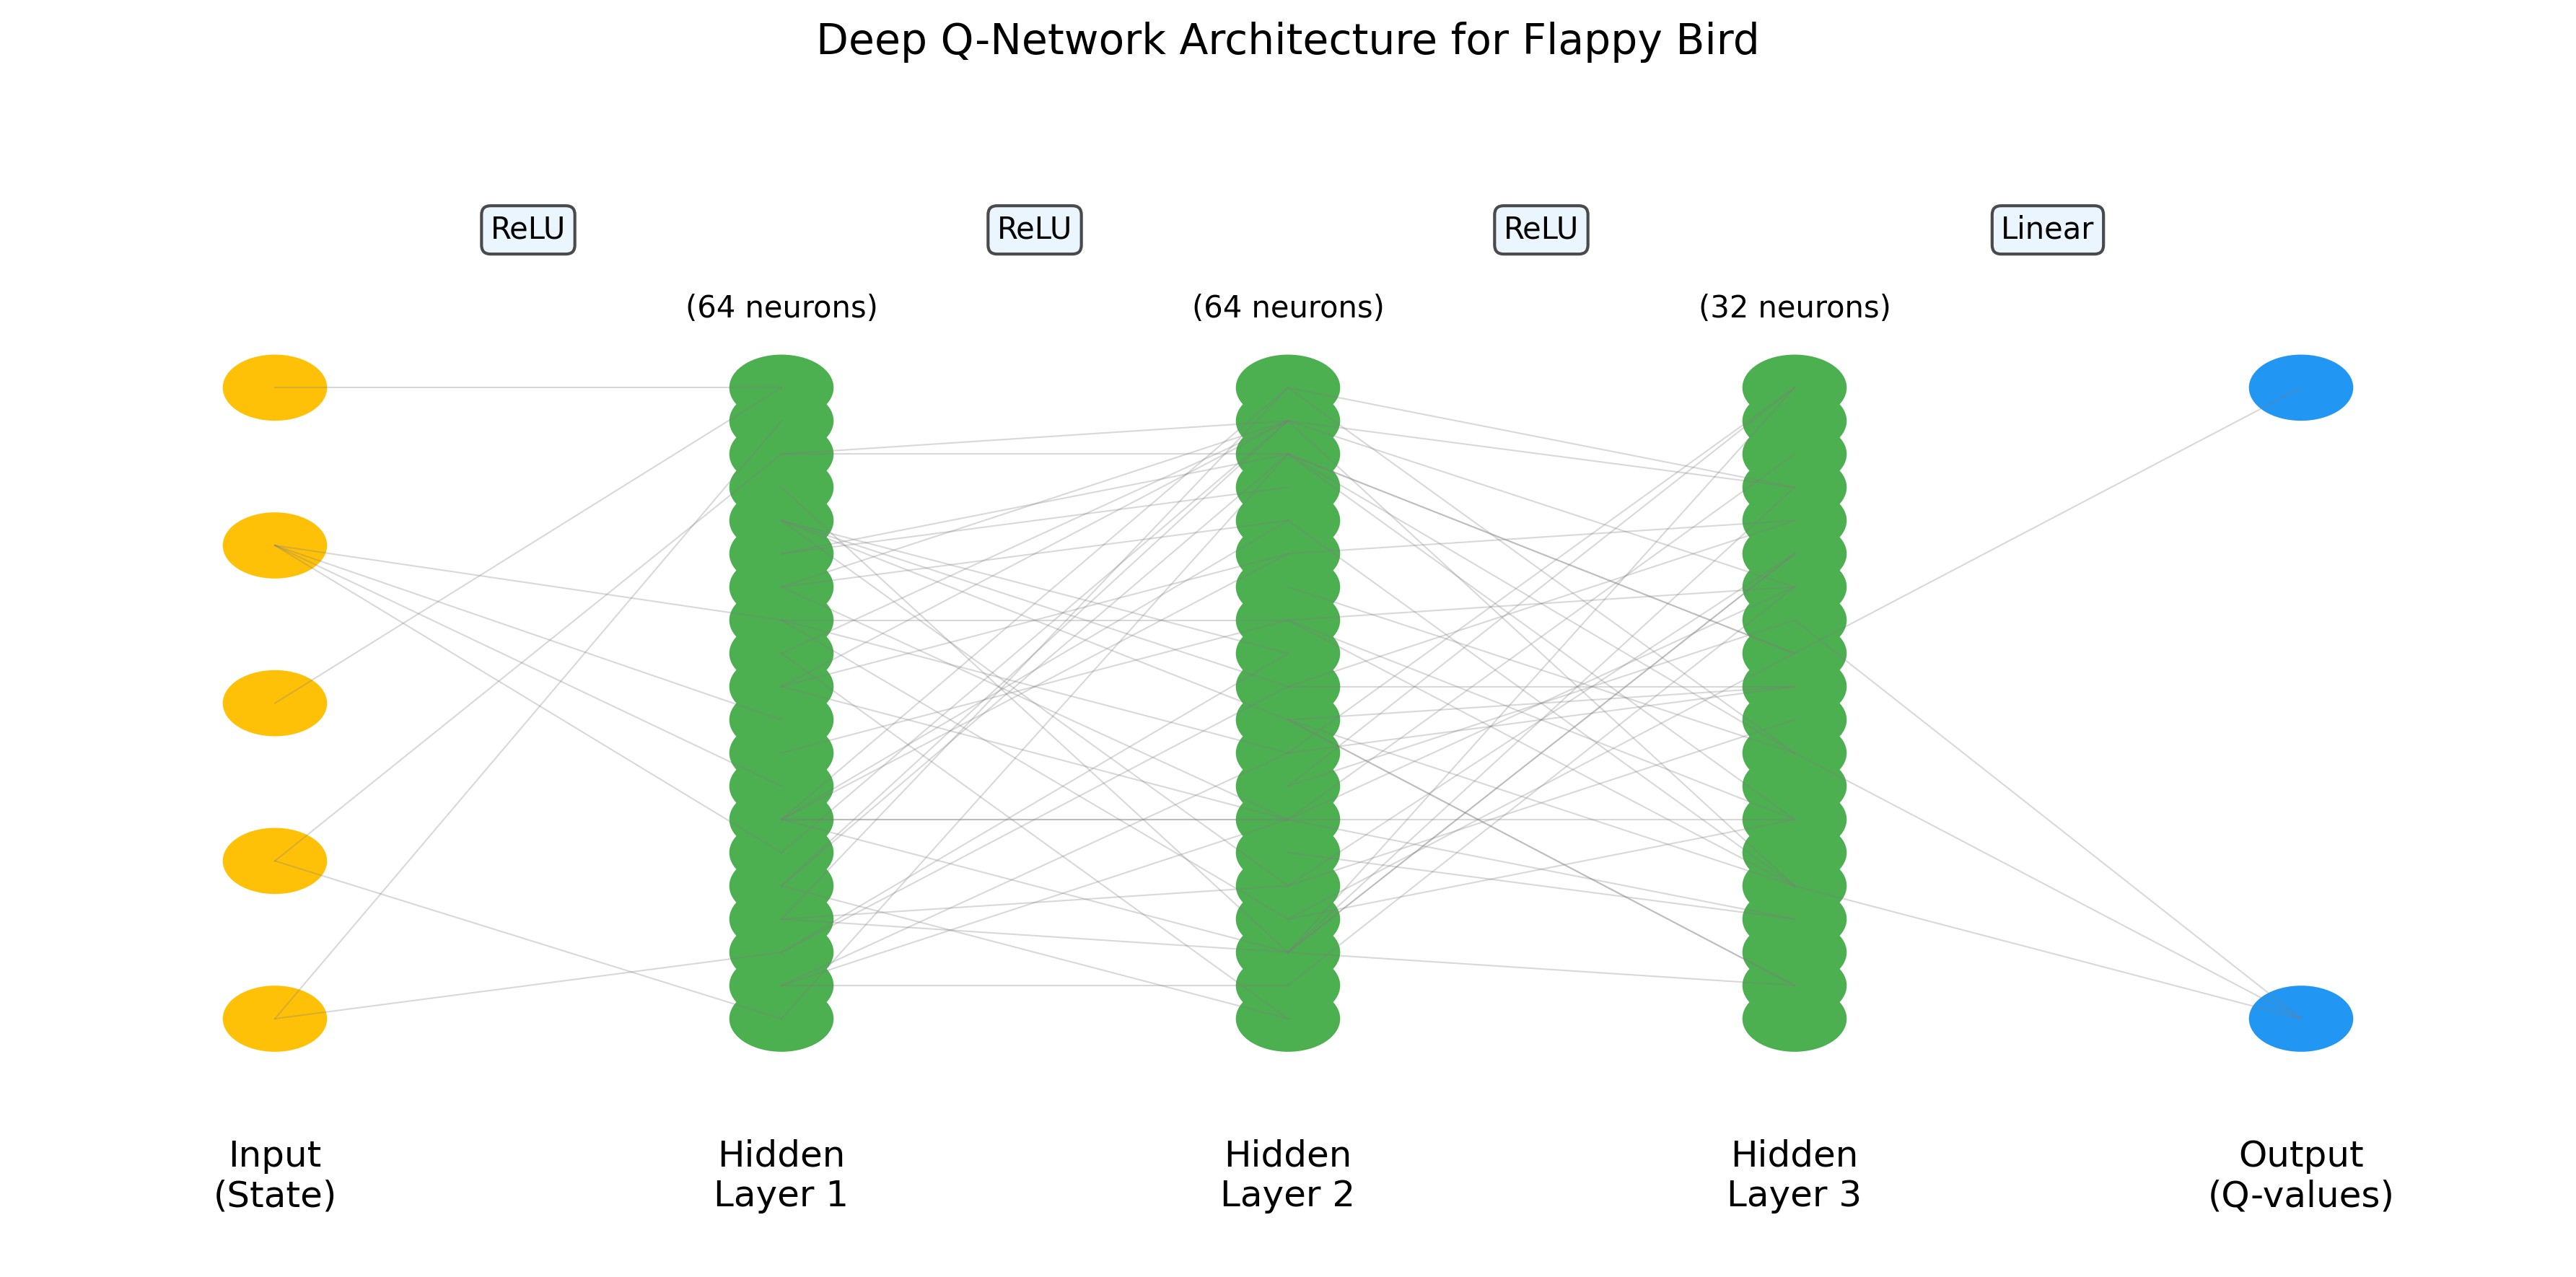
\includegraphics[width=\columnwidth]{/Users/admin/GitHUb/Flappy_Bird_RL/Flappy_Bird_RL/Figures/dqn_architecture.png}
\caption{Deep Q-Network architecture used for the Flappy Bird agent, consisting of an input layer with 5 neurons (state features), three hidden layers with 64, 64, and 32 neurons respectively using ReLU activation, and an output layer with 2 neurons representing Q-values for each action.}
\label{fig:dqn_architecture}
\end{figure}
This architecture was chosen after experimentation with various configurations, balancing representational capacity with computational efficiency. Deeper networks with more parameters did not yield significant performance improvements but increased training time, while smaller networks struggled to capture the complex relationships in the state space. The chosen architecture provides sufficient depth for feature extraction while remaining efficient for real-time inference.

We implemented dropout with a rate of 0.2 after the first hidden layer to mitigate overfitting, particularly important given the relatively small state space and the potential for the agent to memorize specific scenarios rather than learning generalizable strategies. The use of dropout aligns with recent findings by Fujimoto et al. \cite{fujimoto2021minimalist}, who demonstrated the importance of regularization techniques in deep reinforcement learning.

\begin{figure}[!t]
\centering
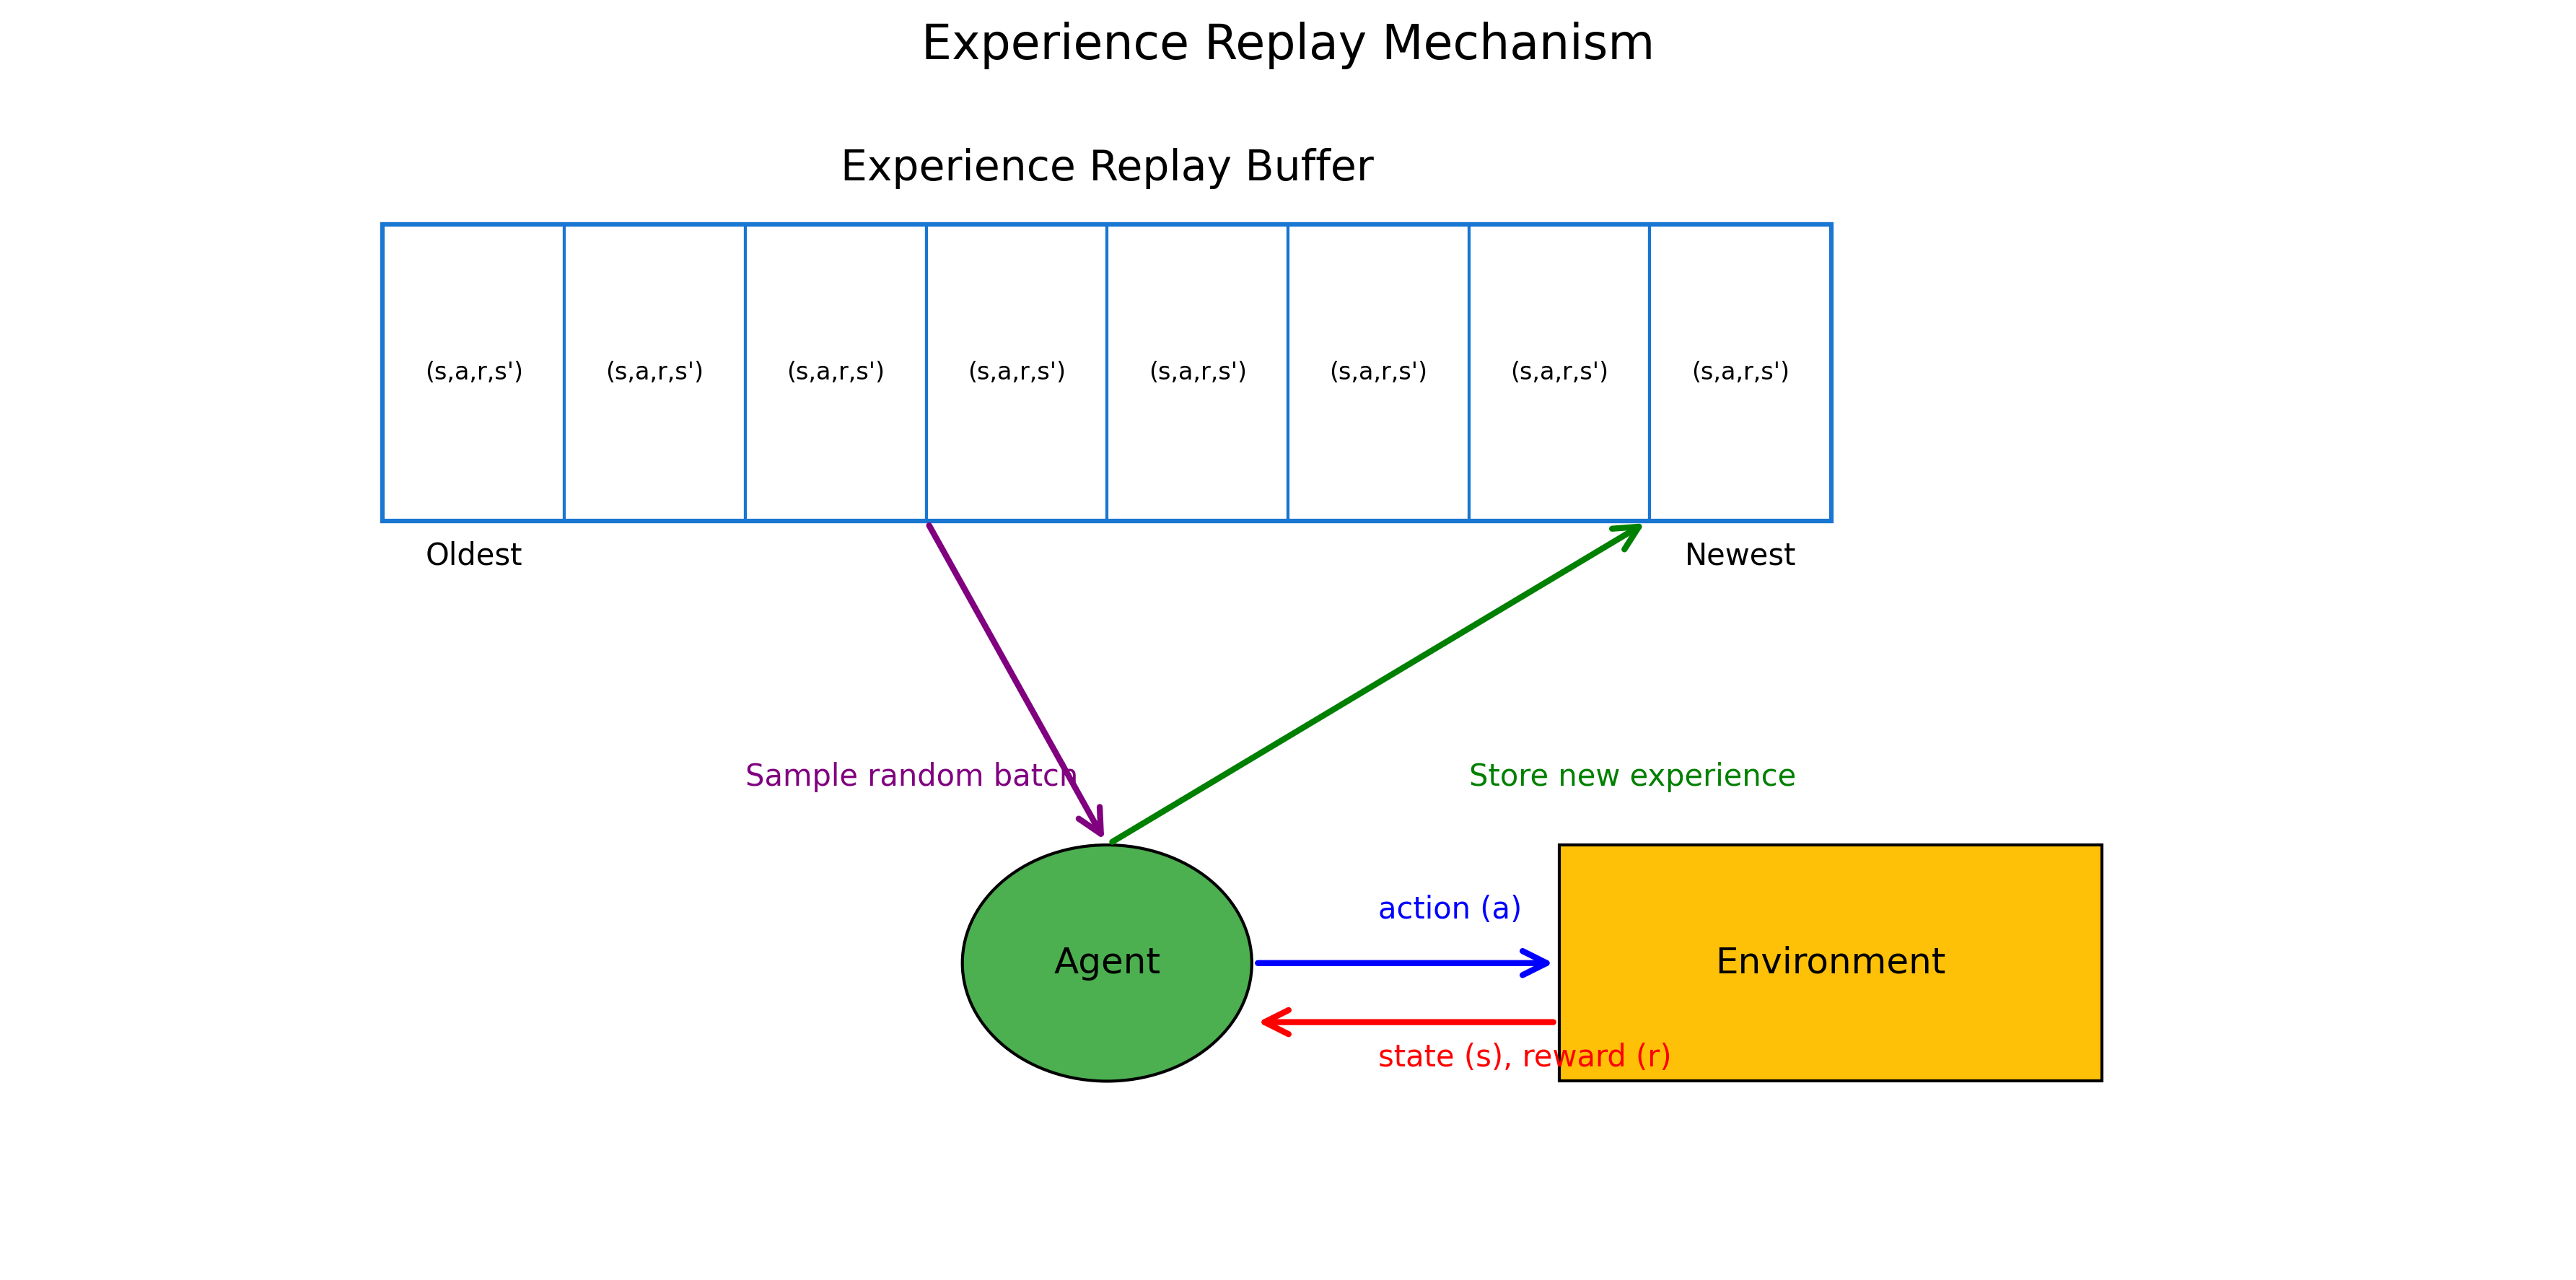
\includegraphics[width=\columnwidth]{/Users/admin/GitHUb/Flappy_Bird_RL/Flappy_Bird_RL/Figures/experience_replay.png}
\caption{Experience replay mechanism: the agent's experiences (state, action, reward, next state tuples) are stored in a buffer, from which random batches are sampled during training to break correlations between consecutive experiences and improve learning stability.}
\label{fig:experience_replay}
\end{figure}

\subsection{Training Procedure}

Our training procedure follows an enhanced version of the standard DQN algorithm. We maintain a replay buffer with a capacity of 10,000 transitions, storing tuples of (state, action, reward, next\_state, done). During training, we sample mini-batches of 32 experiences randomly from this buffer to update the neural network. This experience replay mechanism breaks correlations between consecutive samples and improves data efficiency, a technique that has proven essential for stable learning in deep reinforcement learning \cite{wang2022offline}.

We employ a target network that is periodically updated with the weights from the main network every 10 episodes. This approach provides stable targets for the Q-learning updates, addressing the moving target problem inherent in bootstrapped learning. The update frequency was determined through experimentation, balancing stability with the speed of knowledge transfer.

The agent follows an epsilon-greedy exploration strategy, starting with an exploration rate (epsilon) of 1.0 and decaying it by a factor of 0.9995 after each episode until reaching a minimum value of 0.01. This decay schedule allows for sufficient exploration in the early stages of training while gradually transitioning to exploitation of learned knowledge. The relatively slow decay rate accommodates the precision required in the Flappy Bird environment, where slight variations in timing can significantly impact performance.

We use the Adam optimizer with a learning rate of 0.0005 and a discount factor (gamma) of 0.99 for future rewards. These hyperparameters were determined through a grid search process, prioritizing stability and consistent learning progress. The loss function follows the standard DQN formulation, computing the mean squared error between the current Q-value estimates and the target values derived from the Bellman equation.

The training process consists of 1,000 episodes, with each episode ending when the bird collides with a pipe or the ground. We implemented early stopping with a patience of 100 episodes to terminate training if no improvement in average reward is observed, optimizing computational resources while ensuring sufficient time for learning convergence. This approach aligns with recent work on efficient reinforcement learning training \cite{schulman2023proximal}.

During training, we monitor and record several metrics including episode rewards, game scores (number of pipes passed), exploration rate, and loss values. These metrics provide insights into the learning progress and help identify potential issues such as plateaus or instability in the training process.